

\chapter{Introduction to surface forces}

%Intro
%Surface forces - van der waals, electrostatics, charge screening, DLVO, derjaguin
%hydrodynamics - lubriciating, viscous forces
%brownian 
%Rheology - bulk & translation, shear thickening, friction, industry
%MOVE OUR SYSTEM TO CHAPT4
%Conclision

%Check what I define what a long range force is, what is a short range force is?

%add nomenclature/glossary
%Where is Ue(r) defined ?

%REFERENCES ARE BUGGERED PLEASE FIX BEFORE SENDING OFF TO BE READ!!!

 
\title{Introduction}

The methods of how particles interact with one another have been a longstanding area of interest in physics. As matter encroaches upon one another, there is an interplay of attractive and repulsive forces, which is particularly evident on the microscale of colloidal particles. This transition from repulsive to attractive forces within solutions marks a pivotal point essential for understanding and manipulating the behavior of these colloidal systems. Such knowledge is not only of academic interest but also has significant practical implications, especially in how the rheological properties of solutions can shift given different conditions.

This deep dive into the realm of particle interactions has far-reaching effects that ripple through numerous industries. For instance; the paint and coatings industry, the food industry, the biotech industry and the cosmetic industry, all industries dependant on understanding this interplay where stability and consistency are necessary variables. Furthermore, in the pharmaceutical domain, the implications are even more striking. The efficacy and stability of drugs for health and well-being are fundamentally anchored in these particle behaviors. On a larger canvas, the insights from this research catalyze innovations in smart materials, such as those used in the automotive sector for shock absorption. Beyond the immediate technological triumphs, the environmental aspect is non-trivial. A refined understanding of these interactions paves the way for more sustainable practices and materials, aligning with a global imperative to minimize waste and conserve energy. 

Furthermore, the exploration of particle interactions in colloidal systems extends its significance to the realm of biology, shedding light on the fundamental mechanics of microscopic life. Bacteria, along with a myriad of other microorganisms, can be modelled as simplistic colloids. Their interactions, survival, and behavior in various environments are intricately tied to the same principles of repulsive and attractive forces that govern inanimate colloids. Understanding how these biological colloids interact with each other and their surroundings provides invaluable insights into microbial life. This knowledge is not just theoretical but has practical implications in areas like biotechnology and medicine. For instance, deciphering how bacterial colonies form, adhere to surfaces, disperse, or respond to different environmental conditions can inform the development of new antibiotics and treatments, as well as contribute to the understanding of biofilm formation and its prevention. Additionally, this understanding aids in the development of biosensors and other biotechnological applications where microbial interaction with their environment is key. 

Moreover, the stability and behavior of colloidal suspensions are deeply influenced by these particle interactions. In industries where such suspensions are fundamental, the transition between repulsive and attractive forces directly impacts product stability and performance. Knowledge of where and when this transition occurs is instrumental in developing lasting products, or making a breakthrough in research.

Additionally, these force transitions are central to the study of rheology, particularly concerning shear thickening phenomena. The shift from repulsive to attractive interactions among particles in a shear-thickening fluid is key to understanding the increase in viscosity under stress. A deeper understanding of this transition is critical for uncovering the physics that underlie this behavior, leading to the development of advanced materials with specifically tailored properties.

This PhD, born from a simple desire to understand the forces influencing colloidal interactions on the nanoscale, covers a story started from the simple curiosity of what forces affect colloidal particles when they come in contact with one another. How does this force lead into the wider observed behaviour? Where do these shifts come from and what causes them? Can we model and develop tools to predict their behavior? How do these effects relate to real world life environments and systems? and what breakthroughs can we share with the world? My aim, in truth, was partially to bridge theoretical knowledge with practical application, provide an independent contribution to science and to scale the giant that is modern physics and stand atop the giant's shoulders.

But to first discuss the journey, we must first describe the mountain, and thus this brings us to the fundamental theory behind colloidal particles.

\section{Interparticle Colloidal forces}

The interactions between colloidal particles are predominantly governed by a complex interplay of various forces. These forces dictate the stability, behavior, and ultimate fate of colloidal systems in different environments. Understanding these forces is fundamental to understanding what directs colloidal systems.

The term colloid, coined in 1861 from the Greek word $κόλλα$ (kolla), meaning glue, reflects Thomas Graham's observations of particle aggregation\cite{old_colloid}. Today, a colloid is a mixture comprising a dispersed phase of minute particles or droplets suspended in a continuous phase. The nature of these phases can vary, with examples including solid particles in liquids, liquids in gases (aerosols), and gases in liquids (foams). 

Consider the idea of marbles kept within a liquid. At rest, they would lie upon the bottom of the container, yielding to the force of gravity\cite{Neuton}. However, as you scale down these marbles, to smaller and smaller sizes, the kinetic energy of the system is enough for keep the marbles dispersed within the liquid, due to Brownian motion\cite{Brown}.

At micrometer sizes however, the marbles begin to affect one another; when two marbles are brought together by Brownian motion, provided the interactions between the two of them are attractive, they will attract towards each other, and eventually aggregate, until they are large enough to sediment again. If there is no attraction, or indeed repulsion, between the marbles, they will stay suspended within the solution.

%Interactions between the marble's surfaces, are defined by a few fundamental forces resolving linearly with one another. These interplay of forces, borne from electrostatics, van der Waals and solvation forces, all sum up into a force profile based on distance between the two surfaces.

On the macro scale, these interactions ultimately contribute to bulk properties. As this system is disturbed by external forces, a characteristic relaxation time is observed, dependant on the ions in solution and surface properties of the solid phase particles. 
These properties give rise to the time dependent effects seen in colloidal systems. 

The various interactions between the marble surfaces can be combined to give a force profile, describing the strength of the interaction between the marbles with respect to the distance between them.\cite{FoundColloidBook}\cite{IsGreenBook}

%These force profiles depend upon a number of % intrinsic 
%properties intrinsic to the phenomena. %To define these variables in a broad stroke; the liquid the solid colloid is immersed in (liquid phase properties), the surface properties of the solid phase (solid phase properties) and interactions between same phase particles (same phase interacting properties).


These forces are not merely determined by chemical composition; they are a web of multiple interactions shaped by the colloidal enviromata. Specifically, van der Waals forces, electrostatic interactions, and steric hindrances play significant roles in a solutions stability and organisation. Van der Waals forces, although weak individually, collectively contribute to significant attractions or repulsions at the nanoscale. Electrostatic interactions, governed by the surface charge of the particles and the ionic composition of the medium, further influence particle behavior. Steric hindrance, resulting from the physical size and shape of the particles, adds another layer to this complex interplay.

In addition to these effects solvation forces can also affect colloidal systems. When a colloid is introduced into a solvent, the solvent molecules rearrange around the colloid, leading to a structured layer of solvent molecules at the colloid's surface. This structuring can lead to either attraction or repulsion between colloids, depending on the nature of the colloidal surface and the solvent. Solvation forces are particularly significant in polar solvents like water, where the solvent molecules can form hydrogen bonds and other directional interactions with the colloid surface. Additionally, hydrodynamic forces can affect the distribution of stability of a colloidal system. These forces are governed by factors such as the viscosity of the fluid, the relative velocity between the particle and the fluid, and the size and shape of the particles. Hydrodynamic interactions play a significant role in determining the behavior of colloids under dynamic conditions, such as in suspension flow or by perturbation by a cantilever. These forces arise from the movement of colloidal particles relative to the suspension, resulting in effects like drag and flow-induced reorientation.

Hydrophobic interactions, especially in amphiphilic systems, arise from hydrophobic molecules or groups to aqueous environments. This tendency drives the aggregation of hydrophobic regions, playing a key role in the self-assembly of micelles, vesicles, and the organization of cellular membranes. In these structures, hydrophobic tails cluster away from water, while hydrophilic heads interact with the aqueous environment, creating a dynamic interface. 

When profiling colloidal interactions, it can helpful to imagine it as a dynamic interplay of forces that resolve with one another dependant on distance. As two colloids move towards one another, the forces shift and change between the attractive and repulsive regime. As one expects with a dynamic system such as this, the particle will settle into distinct energy wells. The colloid can be destabilised from this energy well by influential forces overcoming the entrapping energy barriers. These can take the form of kinetic impulses (i.e. a 3rd party physical force applied upon the system), hydrodynamic forces or changes in the suspending medium. In the following sections, each of these forces will be examined in detail, unraveling their individual contributions and collective interplay in shaping the fascinating behavior of colloidal systems


\subsection{Electrostatic interactions} %The repulsive part, unfortunately not in that way.
Electrostatic interactions are fundamental in the study of colloidal systems, governing the behavior and stability of charged particles in various media. The understanding of these interactions dates back to ancient Greek philosophers, but it was the 18th-century physicist Charles-Augustin de Coulomb who formalized the concept. His work on what is now known as Coulomb's Law provided a framework for comprehending the forces between charged particles. This understanding is particularly vital in colloid science, where electrostatic interactions play a key role in the stability of colloids. \cite{halliday2013fundamentals}

In colloidal systems, when two phases mix, ions often arrange along the phase boundary, seeking the lowest energy configuration. This arrangement can create electric fields that induce polarization in nearby molecules, resulting in an electric potential difference between the phases. Such electrostatic phenomena are central to understanding the behavior of colloids, as they influence particle aggregation, stability, and the overall properties of the system. For example, in aqueous colloids, the balance of electrostatic repulsion and attraction among particles can determine whether the colloid remains stable or aggregates.

Coulomb's law provides a basis for understanding these forces in colloidal contexts. The equation demonstrates the force experienced between two electrically charged particles, known as the electrostatic or Coulombic force. The force is governed by the
equation:

\begin{equation}
F = \frac{q_1q_2}{4 \pi \epsilon_r \epsilon_0 r^2}
\end{equation}

In this formulation:
$F$ represents the electrostatic force between the particles.
$q_1$ and $q_2$ are the electric charges of the particles. The force's attraction or repulsion depends on these charges. If both charges are of the same sign (either positive or negative), the resulting force is repulsive, pushing the particles away from each other. In contrast, if the charges are of opposite signs, they attract each other.
$r$ is the distance between the two charged particles. The strength of the force diminishes with increasing distance; it weakens as the square of the distance.
$\epsilon_0$ is known as the vacuum permittivity. It is a measure of the resistance offered by the vacuum of space to the formation of an electric field.
$\epsilon_r$, is the relative permittivity. Unlike in a vacuum, colloidal interactions occur in a medium (such as water), which affects the electric field. The relative permittivity indicates how much the medium reduces the electric field compared to a vacuum. It accounts for the medium's ability to absorb or dampen the electrostatic interactions.

This law thus provides a foundational understanding of how charged colloidal particles interact within a medium. The inclusion of $\epsilon_r$ in the equation adjusts Coulomb's Law from the idealized context of a vacuum to the more complex reality of colloidal systems in diverse environments. In a vacuum, the electric field lines travel without much resistance, but in other mediums like water, air, or any material, these field lines encounter more resistance. This resistance is due to the medium's ability to partially absorb or slow down the electric field. $4\pi \epsilon_0$ is sometimes simplified to the electrostatic constant. 

Charges on surfaces in colloidal systems can arise from several phenomena. The innate surface chemistry of the particles often dictates their initial charge characteristics. For instance, surfaces may naturally possess acidic or basic groups that can gain or lose protons, depending on the pH of the surrounding solution. Additionally, the adsorption of ions from the solution onto the particle surface and the dissociation of surface-bound ions into the solution also contribute to the overall surface charge.

The ionization of surface groups is highly dependent on the pH of the solution. In acidic conditions, basic surface groups tend to gain protons, leading to a positive charge on the surface. Conversely, in basic conditions, acidic surface groups tend to lose protons, resulting in a negative surface charge. This pH-dependent behavior can modify the surface charge characteristics of colloidal particles, thus influencing their stability and interaction in the solution.

Furthermore, the presence of a charge on the colloidal particle surface attracts counter charged ions from the surrounding medium. These counter ions associate towards the charged surface, forming a layer that screens the original surface charge. This is known as charge screening, and is influenced by the concentration and type of ionic salts within the suspending solution. The effectiveness of charge screening plays a significant role in modulating electrostatic interactions between colloidal particles.
\cite{babthes}%33 34 52

\subsubsection{Charge screening}



Charge screening in colloidal systems is a phenomenon where charged surfaces become surrounded by a cloud of counter-ions of opposing charge, leading to the formation of what is known as the electrical double layer. As ionic species diffuse within a solution tending towards a reduction in the free energy of the system, charged surfaces will tend to become surrounded by a cloud of counter-ions of opposing charge. This layer plays a pivotal role in colloidal stability by influencing the electrostatic interactions between particles. 

When oppositely charged ions in the solution approach the charged surface, they tend to reduce the net surface charge, creating an electrostatic potential that decreases with distance from the surface. This process leads to a distribution of ions, known as the Gouy-Chapman-Stern model, which describes the behavior of ions near the charged surface. As such the concentration, charge and valence of the ionic salts will change the repulsive forces upon interacting colloids.\cite{?}

\begin{figure}[h]    
        \begin{center}
          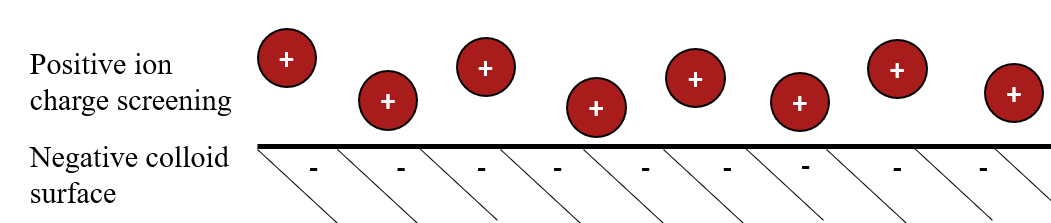
\includegraphics[width=110mm]{chapter1/ioncloud.PNG}
\end{center}
\caption{A schematic of counter ion distribution under the Gouy-Chapman model. This demonstrates how positive counter ions will arrange themselves around a negative surface.}
\label{fig:ioncloud}                
\end{figure}

%Foundations of colloid science
These ions are subjected to an electrostatic potential ($\Psi$) as they get closer towards the oppositely charged surface. The positive counterions (see fig \ref{fig:ioncloud}) are attracted by the electric field generated from the negatively charged surface producing a potential seen in fig \ref{psi}. 

\begin{figure}[h]    
        \begin{center}
          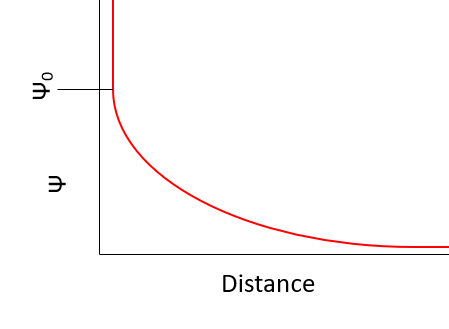
\includegraphics[width=80mm]{chapter1/psi.PNG}
\end{center}
\caption{The Electrostatic potential of a counter ion, where distance is the distance between the negative surface and positive ion.}
\label{fig:psi}                
\end{figure}

%Volta and Galvani potentials (inner and outer) - though maybe not exactly needed. Mostly interested in the double layers interacting.

In addition to the electrostatic attraction, ions in colloidal systems are also subjected to thermal motion. This thermal motion leads to a random distribution of ions uniformly, counterbalancing their electrostatic attraction to the charged surface. As a result, the concentration of counterions decreases with increasing distance from the surface. This leads to the formation of the diffuse electrical double layer which also includes the Stern layer. 

The concept of the electrical double layer has been explained through several historical models. The Helmholtz model, proposed in 1853, suggested a simple planar distribution of charges directly opposite the surface charge, akin to a parallel plate capacitor. This distribution is a function of the distance away from the surface, and thus surface charge. While this model provided a basis of understanding the interactions between solvent ions and surface charges as a function of distance, it was unable to account for the effects of kinetics on the system.

The Gouy-Chapman model developed between 1910 and 1913 introduced a more dynamic understanding. This model considered the impact of thermal motion, leading to a diffuse distribution of ions. It relies on the linearized Poisson-Boltzmann equation, which correlates the electrostatic potential with the charge density around the colloidal particle, allowing for a theoretical description of the diffuse layer. This model assumes a uniform surface charge and a homogeneous dielectric constant for the solution, implying that ions form a diffuse point charge region rather than discrete binding sites.

% linearized Poisson-Boltzmann equation 
%\begin{equation}
%\frac{d^2 \psi}{dx^2} = \kappa^2 \psi
%\end{equation}
%psi represents the electric potential.
%dx is the differential element in space (in one dimension).
%\kappa is the inverse of the Debye length (a parameter that describes the thickness of the electric double layer and depends on the ionic strength of the solution).

Within this region there is a volume of liquid that is unique to the bulk properties of the liquid phase. This region with a higher concentration of counter ions is called the Helmholtz region and is further split up into two parts. The closest to the surface being the inner Helmholtz plane - where ions are adsorbed onto the surface, and the outer Helmholtz layer contains solvated ions. Afterwards the diffuse layer is made up of unbound free ions influenced by Brownian motion.

The Diffuse layer is characterized by a gradual reduction in counterion concentration until it reaches the bulk concentration level. The Stern layer comprises specifically adsorbed ions in the inner Helmholtz plane and more loosely associated solvated ions in the outer Helmholtz plane. This layer represents the initial structuring of ions influenced by the surface charge before transitioning into the more diffuse arrangement of the bulk solution." The distribution of ions in this layer is highly dependent on the electrolytes present in the solution.

\begin{figure}[h]     %Insert a figure as soon as possible
        \begin{center}
          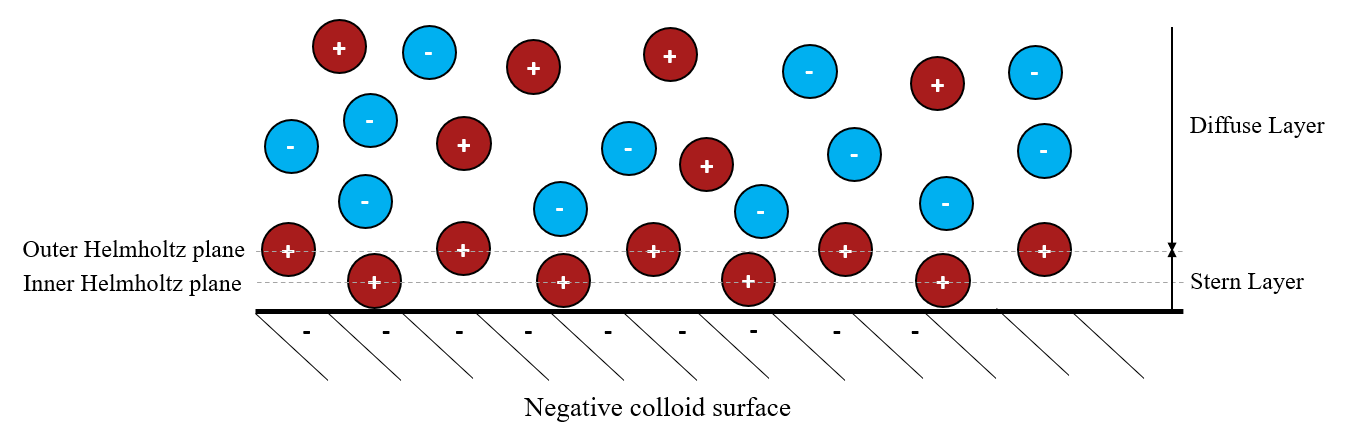
\includegraphics[width=110mm]{chapter1/SternLayer.PNG}
\end{center}
\caption{The Electrical double layer model highlighting the transition between the Stern and diffuse layers.}
\label{fig:Stern}                 % Reference label to the figure.
\end{figure}

The measurement of the distance beyond which the electrostatic force between charged particles is insignificant is known as the The Debye length ($\lambda_D$). It represents the distance over which the electrostatic influence of a collodial surface charge extends into the solution. The Debye length is given by:

\begin{equation}
\lambda_D = \kappa^{-1} = \sqrt{ \frac{ \epsilon_r \epsilon_0 k_B T}{2Z^2 e^2 n_b}}
\end{equation}

Where $\epsilon_0$ is the vacuum permitivity, $k_B$ is boltzmann constant, T is  Temp in K) 
$\epsilon_r$ is the relative dielectric constant, e is the elementary charge, Z is the charge number of the ions in solution and $n_b$ is the number density of the ions. %(units $\frac{1}{m^3}$)
The number density is given by:
%(LiCl, NaCl etc at 1:1 electrolytes, so Z=1, if you have multiple types of ions in solution you have to sum up the different contributions, but we don’t need to worry about this)
\begin{equation}
n_b = N_A \frac{moles} {Volume}
\end{equation}

Where $N_A$ is Avogadro's constant. This can be further simplified to:

\begin{equation}
 \lambda_D = \kappa^{-1} = \sqrt{ \frac{ \epsilon_r \epsilon_0 k_B T}{2000N_A e^2 I}}
\end{equation}

Where I (the ionic strength) is calculated using:

\begin{equation} 
I = \frac{1}{2} \Sigma c_i z_i^2
\end{equation}

The Debye length measures the effective thickness of this diffuse layer. It represents the distance beyond which the electrostatic influence of the surface charge becomes insignificant. The Debye length is dependent on factors such as temperature, the dielectric constant of the medium, and the ionic strength of the solution. The ionic strength, in turn, affects the distribution and concentration of ions in the diffuse layer.

 %what? Helmholtz was before, not after.
%1853 Helmholtz -> Gouy-Chapman 1910 -> Stern 1924 -> Grahame 1947 -> BDM 1963 -> Trasatti/Buzzanca 1971 -> Conway 1975/80ish -> Marcus 1992 (looks quantum? Electron jump probabilities)
%Rough timeline - not all individual theories
%Overbeek (1952) ->

%and electrostatics, but that's not unique? 

\subsubsection{Electrostatic repulsion}

%Expand upon double layer interactions

Electrostatic repulsion plays a significant role in maintaining the stability of colloidal suspensions. When two colloidal particles in a suspension approach each other, their respective electrical double layers begin to overlap and repel one another. Without this repulsion attractive van der Waals forces (detailed in the next section) would dominate, leading to particle aggregation. The nature of this electrostatic repulsion is closely linked to the presence of the electrical double layer surrounding each colloidal particle. As detailed previously, the double layer consists of surface-bound charges and a diffuse layer of counterions, which create a repulsive force when two colloidal particles approach each other. This repulsion counterbalances the attractive van der Waals forces, thereby  stabilizing the colloidal system..\cite{?} The electrostatic energy of this repulsion is given by:

%\begin{equation} %This can't be right??
%U_E (r) = 4\pi\epsilon R \Psi^2_{0} \epsilon_0 e^{-\kappa h}
%\end{equation} %WRONG

\begin{equation} %WHERE DID THIS COME FROM!?!?!?
U_E(r) = \frac{\epsilon_r \epsilon_0 \Psi_0^2}{\kappa} e^{-\kappa h}
\end{equation}

\( U_E(r) \) represents the electrostatic repulsion energy as a function of the distance (\( h \)) between the particles. \( \epsilon_r \) is the relative permittivity of the medium, and \( \epsilon_0 \) is the vacuum permittivity. \( \Psi_0 \) is the surface potential of the colloidal particles. \( \kappa \) is the inverse Debye length   determines how quickly the potential decays with distance, related to the thickness of the electrical double layer. \( e^{-\kappa h} \) is an exponential term that describes how the repulsion decreases with the distance between the particle surfaces. \cite{OHSHIMA200218} \cite{behrens2001charge}

The Debye length is a key factor that governs the range of electrostatic interactions. In solutions with high ionic strength, the Debye length is shorter, leading to a more compressed double layer. Consequently, the electrostatic repulsion decreases more rapidly with distance, allowing particles to come closer before experiencing significant repulsive forces. In contrast, in low ionic strength solutions, the Debye length is longer, and particles experience repulsive forces over greater distances, contributing to the stability of the suspension by preventing aggregation.

The other factor that affects colloids in suspections is the attractive component. This component derives from Van der Waals forces.

%\begin{equation} %~1 - 100 (50-100 silica ph9) (find ref)
%\Psi_0 \approx \frac{\epsilon_r \epsilon_0 \kappa}{\sigma}
%\end{equation}
%Find approx sigma value
%where does this come frommmmmmmmmmmmmm


%w(r) is Joules, ~ 8x10^-19J, kT is 5x10^-21J. Stronk.

%lennard jones potential here?

\subsection{Van der Waals Forces}

%Honking

The strongest attractive forces acting on the solid phase of a colloidal system are described by van der Waals theory. Originally recognized by Johannes Diderik van der Waals in 1873 \cite{vanderWaals}, these forces were further refined by London in 1930 \cite{London} almost 60 years later, leading to the concept of London dispersion forces. 

Van der Waals forces can be categorized into three types: Keesom forces (permanent dipole-permanent dipole interactions), Debye forces (permanent dipole-induced dipole interactions), and London dispersion forces (induced dipole-induced dipole interactions) \cite{sciDirBook}. 

Keesom forces derive from the permanent charge nature of atoms, where a static dipole induces an attraction between two particles, due to their stable differences in charge (see fig \ref{fig:keesom}). These forces follow an inverse sixth power law (\(1/r^6\)) with respect to the distance between the dipoles, reflecting their short-range nature in colloidal systems.

\begin{figure}[h!!!!!!!!!!!!!!!!!!!!!!!!!]     %Insert a figure as soon as possible
        \begin{center}
          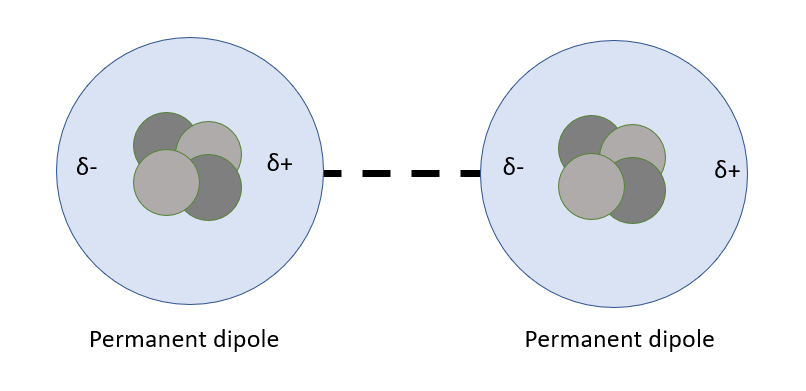
\includegraphics[width=110mm]{chapter1/keesom.PNG}
\end{center}
\caption{A basic schematic of Keesom interacting forces.}
\label{fig:keesom}                 % Reference label to the figure.
\end{figure}

Debye forces result from the influence of an instantaneous dipole on a permanent 
the interaction between the electronic fields results in a force between the dipoles, initially without a dipole moment. This interaction, illustrated in Figure \ref{fig:debye}, stems from the influence of the fluctuating electronic field of the permanent dipole on its neighboring particles.

\begin{figure}[h!]     %Insert a figure as soon as possible
        \begin{center}
          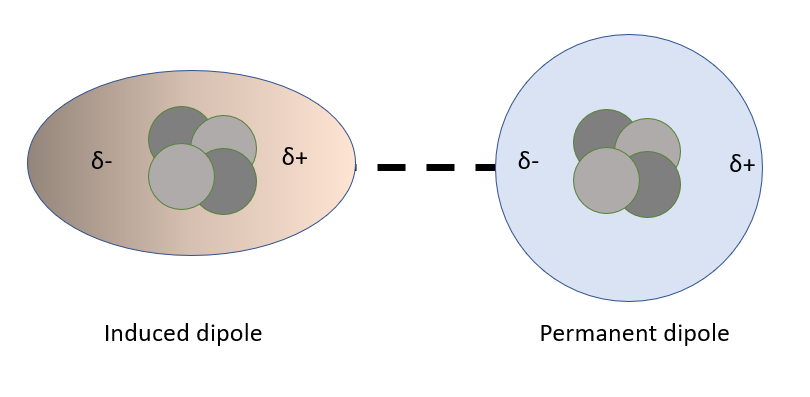
\includegraphics[width=110mm]{chapter1/debye.PNG}
\end{center}
\caption{A basic schematic of Debye interacting forces.The orange dipole represents an non permanent sudden gradient.}
\label{fig:debye}                 % Reference label to the figure.
\end{figure}

Dispersion forces (see fig \ref{fig:dispy}) act between all atoms and molecules, even those in neutrally charged elements. These forces arise due to fluctuations in electron density around the nucleus, as a consequence of the Heisenberg uncertainty principle.\cite{heisenberg1927uber} \cite{griffiths2005} This dispersion force is caused by an electronic charge flux inducing a dipole moment and is unique in that it does not require the presence of permanent dipoles, unlike Keesom and Debye forces, which depend on their permanent dipole properties and the nature of the medium. \cite{IsGreenBook} To understand the origin of these forces, consider an atom with a time-averaged dipole moment of zero. Fluctuations in the electron density around the nucleus result in a non-zero instantaneous dipole moment. This fluctuating instantaneous dipole moment generates a fluctuating electric field on any neighboring neutral atoms. The interaction between the instantaneous dipole moment in one atom and the induced dipole in another, averaged over orientation to account for the fluctuating nature of the instantaneous dipole, gives rise to an attractive interaction between the two atoms. 

\begin{figure}[h!]     %Insert a figure as soon as possible
        \begin{center}
          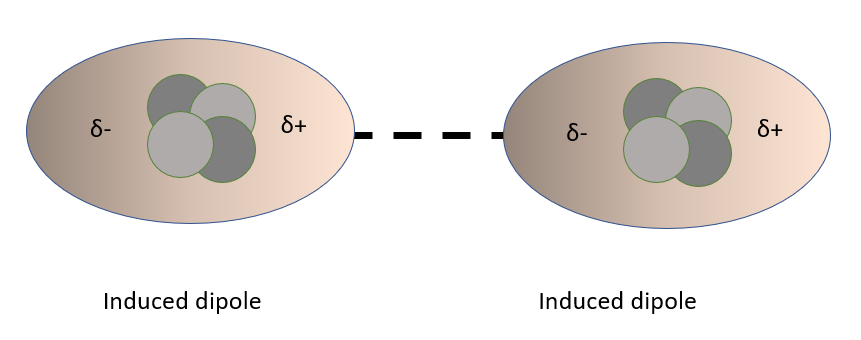
\includegraphics[width=110mm]{chapter1/London.PNG}
\end{center}
\caption{A basic schematic of dispersion interacting forces.}
\label{fig:dispy}                 % Reference label to the figure.
\end{figure}

The intensity of the induced electric field from instantaneous dipole moments decreases with distance, which can be described by the equation:
\begin{equation}
E_{\text{ins}} \propto \frac{1}{r^3}
\end{equation}
This reflects that as the distance (\(r\)) increases, the intensity of the induced electric field, generated due to instantaneous dipole moments, diminishes significantly.

The induced dipole moment is proportional to this electric field, where the proportionality constant is the polarizability (\(\alpha\)) of the second atom:
\begin{equation}
p_{\text{ind}} \propto \alpha E_{\text{ins}}
\end{equation}
Here, \(p_{\text{ind}}\) represents the induced dipole moment, which is formed in response to the external electric field (\(E_{\text{ins}}\)). The polarizability, \(\alpha\), measures how easily the electron cloud of the atom is distorted to form this dipole moment.

Consequently, the interaction energy between the two atoms, which arises from these induced dipoles, follows an inverse sixth power law with respect to the distance:
\begin{equation}
U \propto \frac{\alpha}{r^6}
\end{equation}
This equation signifies that the interaction energy (\(U\)) decreases very rapidly as the distance between the atoms or molecules increases, following an inverse sixth power law. This rapid decrease is important, as it places a high impact on the distance between particles influencing the resulting attractive force.

These equations collectively describe the fundamental mechanism of dispersion forces, highlighting how forces arise from instantaneous dipole-induced dipole interactions and lead to an attractive force between atoms or molecules. This attraction occurs even in the absence of permanent dipole moments, leading to an attractive force seen between colloidal particles.

The stability of colloids is significantly influenced by Van der Waals forces, which govern the attractive interactions between particles. These forces can lead to particle aggregation especially when they overpower repulsive forces such as electrostatic interactions in charged colloids. The phenomenon of aggregation resulting from dominant Van der Waals attractions can reduce colloidal stability, potentially causing sedimentation or phase separation. 

These van der Waals forces, comprising Keesom, Debye, and London dispersion forces, play a pivotal role in the behavior of colloids. Their predominance in short-range interactions is essential for understanding the stability and dynamics of colloidal systems \cite{colloid_review1}\cite{lilBlueBook}\cite{IsGreenBook}\cite{FoundColloidBook}. These overall forces can be expanded to describe the full positive effect on colloids by the following equation \ref{Hammy}: 

%Fill out - T
\subsubsection{Mathematical basis of dispersion forces} %inseperable

The Van der Waals interaction energies in colloidal systems can be represented mathematically through various equations. Two such expressions for the Van der Waals potential energy (\(U_{vdW}\)) are:

\begin{equation}  %Alternative - from excel model paper (Nano focused, misses out on larger particles?) R must be distance then?? (nanocoatings practice and principles)
U_{vdW} (r) = - \frac{A}{12hkT} \times \frac{r}{R}
\label{Hammy}
\end{equation}

\begin{equation}
U_{vdW} (r) = - \frac{A}{12\pi} \left( \frac{R}{r}\right)^2
\label{VDWeqn}
\end{equation}


In these equations, \(U_{vdW}\) is the attractive cohesive energy, \(A\) is the Hamaker constant, \(R\) is the radius of the colloidal particle, and \(r\) is the distance between the two particles. Equation \ref{Hammy} is derived under specific conditions and is more applicable to nano-scale interactions, whereas Equation \ref{VDWeqn} can be used for larger particle interactions highlighting the modification of these models needed for different size regimes. The Hamaker constant (\(A\)), a fundamental parameter in these equations, is influenced by the material properties of the colloidal particles and the medium. The Hamaer constant is given by:

\begin{equation} %Foundation of collodial science
A = \pi^2 C p_1 p_2
\end{equation}

Where C is the interaction parameter, given by the coefficient in the particle-particle pair interaction. $p1$ and $p2$ are the number densities of two interacting kinds of particles.\cite{?} C is calculated by:

where \(C\) is the interaction parameter, given by the coefficient in the particle-particle pair interaction, and \(p1\) and \(p2\) represent the number densities of the two interacting particle types. \cite{FoundColloidBook} The interaction parameter \(C\) is determined as follows:


\begin{equation}
w(r) = - \frac{C}{r^6}
\end{equation}

where \(w(r)\) denotes the pair interaction energy between two particles. 

One striking element of these interactions is their short range - their significance only felt up to tens of nanometers. This is significant in colloidal systems particularly in solvent environments, where the Hamaker constant (\(A\)) assumes characteristic values depending on the colloidal and solvent properties. The interaction range significantly influences colloidal properties such as aggregation, stability, and rheology, highlighting the importance of understanding these forces.\cite{?} %Great where did my citation go

\section{The Interplay of Attractive and Repulsive Forces on Colloidal Systems}

The intricate balance between attractive and repulsive forces plays a pivotal role in determining the stability of colloidal systems. This interplay between Van der Waals forces and electrostatic interactions, forms the theoretical foundation of colloidal behavior. While Van der Waals forces tend to draw particles together, potentially leading to aggregation, it is the counteracting electrostatic repulsion that often dictates whether a colloidal system remains stable or not. The stability of colloids thus depends on the equilibrium between these competing forces. Delving deeper into this complex interaction, the subsequent sections will explore the Lennard-Jones potential and the DLVO theory. The Lennard-Jones potential provides a fundamental model for understanding the balance of attraction and repulsion at a molecular level, while the DLVO theory offers a comprehensive framework that elucidates how this equilibrium contributes to the overall stability of colloidal systems and provides the main theoretical basis of understanding this practical thesis.

\subsection{Lennard-Jones potential} %Mostly bulk? Not sure if needed.
%Give a history lesson not a maths lesson

The Lennard-Jones potential stands as an introduction in modeling intermolecular forces within colloidal systems. By illustrating the equilibrium between attractive and repulsive forces, this model provides a fundamental understanding of how colloids arrange themselves at a characteristic distance, giving rise to collodial stability.

\begin{figure}[h!!]     %Insert a figure as soon as possible
        \begin{center}
          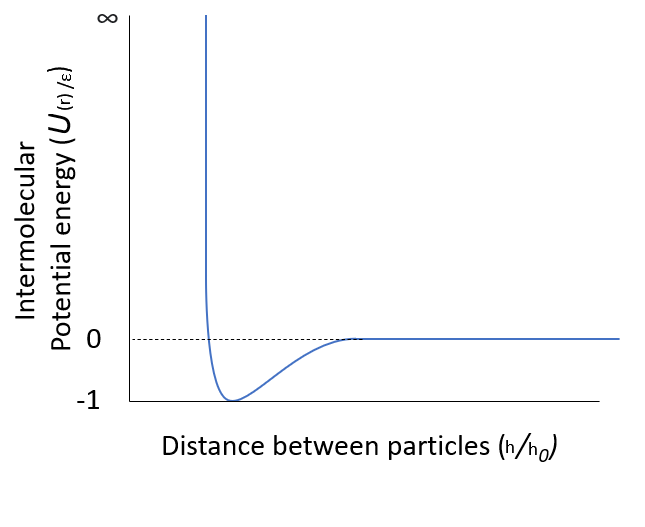
\includegraphics[width=100mm]{chapter1/Lennard's potato.PNG}
\end{center}
\caption{The Lennard-Jones potential function. The potential energy between the two particles is given as a function of distance. As the particles begin to get closer, the experience attraction. As the distance between the two shortens, the attraction eventually gives way to a infinitely increasing repulsive force.}
\label{fig:potato}                 % Reference label to the figure.
\end{figure}

The Lennard-Jones potential offers a useful visual representation of intermolecular forces. This model is particularly useful for visualizing the variation of potential energy as a function of the distance between particles. At the nadir of this curve lies the energy well, a concept that illustrates the balance between attractive and repulsive forces, and demonstrates the optimal distance location between interacting particles under no external forces. This balance occurs at a specific inter-particle distance where the system achieves its minimal potential energy and thus equilibrium state.

The graphical representation of the Lennard-Jones potential (see Figure \ref{fig:potato}) serves as a visual representation of the concepts discussed earlier, combining the effects of electrostatic repulsion and Van der Waals attraction into a singular curve. The curve demonstrates how these two forces interplay to create a stable configuration at the energy well. This model also shares the form of an atomic force microscopy (AFM) force curve, further emphasizing its practical relevance. 

%Pauli - electron spin repulsion (possible to have two electrons on the same quantum state due to electron shell overlap - this leads to repulsion)

This originally sought to model interactions between two noble gas atoms by describing Pauli repulsion coupled with an attractive long range term. This provides a simplistic view by assuming all interactions between all particles are the same and thus the solution is homogeneous. This is done by summing the contributions from all particles interacting with one another. However, this simplification also introduces limitations. The Lennard-Jones potential does not account for solvent effects and assumes particles are in a vacuum. Additionally, it overlooks the role of charge, which is particularly important when ions are present in the solvent. In reality, particles immersed in a solvent experience modified forces leading to a reduced attractive interaction than vacuum conditions.
\cite{lilBlueBook}
%For each interaction the attraction is given by the Van der Waals attraction (See equation \ref{VDWeqn}). The repulsive term is given by:



%Further simplification can be done in the following form 
%rewrite: Which can be simplified to:

%\begin{equation} %Basic principles of colloid science
%U = 4 \epsilon_{min} \left[\left(\frac{r_0}{r}\right)^{12} - \left(\frac{r_0}{r}\right)^6\right]
%\end{equation}



%This removes the need for the $A$ and $B$ constants, instead expressing the relationship using the depth of the potential well ($\epsilon_{min}$) and the distance at which the potential is 0 ($r_0$).  

These limitations highlight the need for more comprehensive models which leads us into DLVO theory. DLVO theory, which integrates electrostatic repulsion and Van der Waals attraction, addresses some of the shortcomings of the Lennard-Jones potential by considering the specific conditions of colloidal systems, including the presence of a solvent and the role of ionic strength.\cite{} %Find a paper to support this, just in case. What do you mean you don't have one past me??

%In order to improve upon the basics laid out here, these factors need to be considered mathematically. To this end, electrostatics are introduced and considered.

\subsection{DLVO theory}



DLVO theory, named after its developers Derjaguin, Landau, Verwey, and Overbeek in the mid-20th century, describes the complex interplay of forces within colloidal systems. This theory represents a dance of forces where electrostatic repulsions \( U_E(r) \) and van der Waals attractions \( U_{\text{vdW}}(r) \) continually sway between dominance, impacting the stability and behavior of colloids.\cite{DLVOorign} \cite{Origin2V} \cite{DERJAGUINORIGIN}


The context of the initial theory was done upon lyophobic colloids, which is to say a collodial suspension of particles in a medium that does not precipitate. Particles are prevented from merging (coalescence) and separating via repulsive forces present between one another, and as a result in an equilibrated state it is stable. This repulsion is produced due to the repulsive electrostatic forces described in 1.1.2, present due to the surface charges of the colloid. The attractive forces of the equation result from van der Waals forces present from the electron distribution of the atomic core, from the molecular surface of the colloid, described in 1.1.2.\cite{DLVOthesis}

These two forces combine to produce a defining interaction potential:

\begin{equation}
U_{\text{DLVO}}(r) = U_{\text{vdW}}(r) + U_{E}(r)
\end{equation}

This equation expresses the total interaction potential within DLVO theory, where \( U_{\text{DLVO}}(r) \) is the sum of van der Waals and electrostatic forces at distance \( r \). This interplay can be visually illustrated by \ref{fig:DLVO}.


%I'm not green with it
\begin{figure}[h]     %REDO THIS CURVE IT IS BAD AND YOU'RE NOT COMFORTABLE WITH IT Oops ran out of time lol
        \begin{center}
          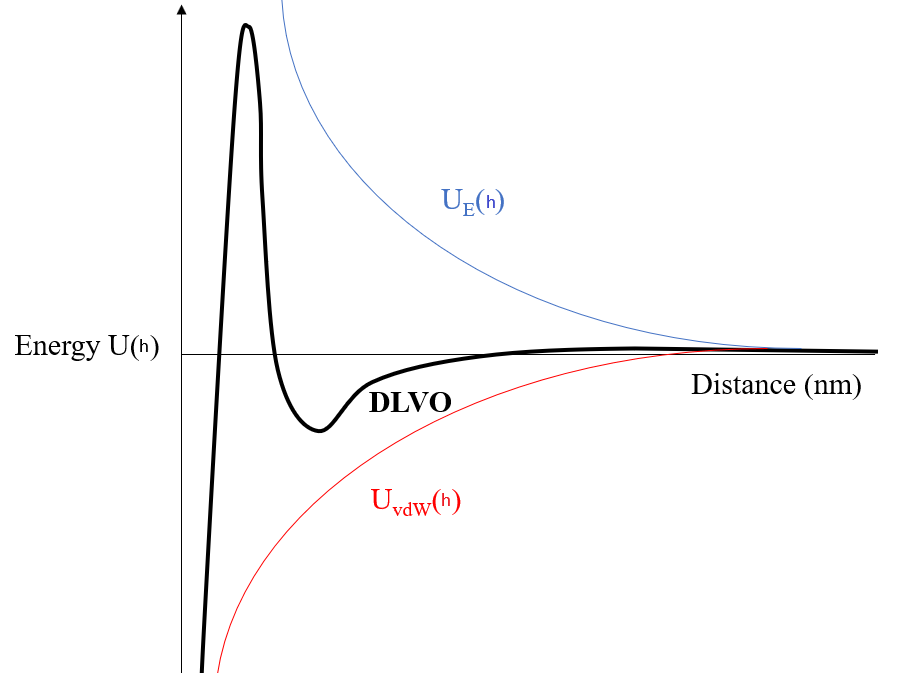
\includegraphics[width=110mm]{chapter1/DLVO.PNG}
\end{center}
\caption{A graphical demonstration of the competing forces between collodial particles. The electrostatic repulsion ($U_E(r)$) and the van der Waals attraction $U_{vdW}(r)$ combine together the sum interplay known as DLVO theory (bold line).}
\label{fig:DLVO}                 % Reference label to the figure.
\end{figure}

One key feature of DLVO is the repulsive barrier that is seen from the initial dip. This energy barrier prevents colloids from agglomerating. The Van der Waals forces are generally attractive due to the nature of their interactions at longer ranges, giving rise to the inital dip, before the electrostatic repulsion dominates, producing said barrier. However, after this energy barrier is broken, the attraction descends to infinity, demonstrating a very strong attraction. If this barrier is substantial enough to offset the kinetic energy from Brownian motion, colloidal stability is achieved. In the absence of sufficient repulsion, particles may overcome this barrier, leading to aggregation.

While DLVO has proven itself a functional and applicable model for the description of interacting colloids, there remains a few assumptions that can limit its accuracy. DLVO assumes that the interacting surfaces is perfectly flat, expanding in all directions, and that the surface charge density is uniformly distributed along said surface. Additionally, it assumes that the surface electric potential is constant, and that any counter ions remain static and uniformly distributed too, with any interactions between said ions or solvent being purely born from their dielectric constant. While some of these assumptions aren't true for particle-particle interactions, DLVO holds up as one of the main theories for predicting interactions. \cite{particledep} \cite{effectHetSurf} \cite{colloidDepKin} \cite{chemDiscCharge} \cite{DLVOreview} 

However since this assumes that the interacting objects are flat planes, and not spherical objects. In order to apply this theory to spherical colloids their geometry has to be considered. To this effect the Derjaguin approximation is used to approximate the DLVO force between differing geometries. This approximation adapts DLVO principles to spherical geometries, allowing for a more accurate representation of force interactions in many real-world colloidal systems. 

\subsubsection{Derjaguin approximation}

The Derjaguin approximation is a useful approximation in colloidal science, particularly for calculating the interaction forces between particles with non-linear geometries. It simplifies the complex interactions in colloidal systems to a more manageable form, particularly useful when dealing with spherical particles or sphere-plane interactions.

%THIS IS DEYAGUIN APPROX PLS
In the Derjaguin approximation, The force $F$ experienced by two interacting spherical colloidal particles is given by the free energy ($W$) of two plates per unit area with respect to the distance between the two ($h$). This relationship is expressed as:

\begin{equation} %colloid.ch
F(h) = 2 \pi r_{eff} W(h)
\end{equation}

$W(h)$ represents the interaction energy per unit area between two surfaces as a function of their separation distance $h$, $R_{eff}$ is the effective radius calculated using the radii of the two particles, given by:

\begin{equation} %colloid.ch
r_{eff} = \frac{r_1r_2}{r_1 + r_2}
\end{equation}

Where $r_1$ and $r_2$ are the radii of the two interacting particles. In systems where the radius is homogeneous $r_{eff}$ can be modified to $\frac{r}{2}$. For a system with a sphere and a plane, $r_{eff}$ can be altered to simply equal $r$.

\begin{figure}[h]     %REDO THIS CURVE IT IS BAD AND YOU'RE NOT COMFORTABLE WITH IT
        \begin{center}
          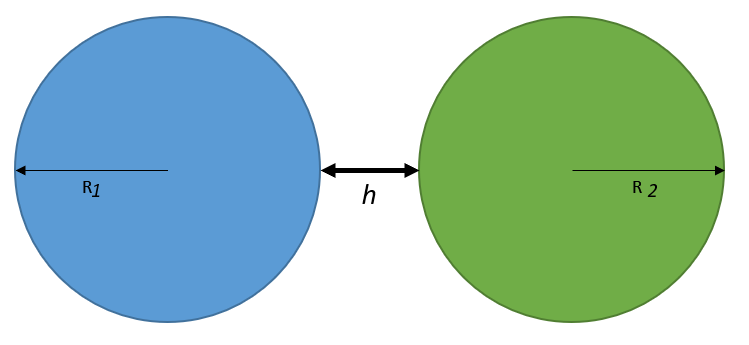
\includegraphics[width=110mm]{chapter1/h_graph.PNG}
\end{center}
\caption{A graphical representation of $h$.}
\label{fig:h_graph}                 % Reference label to the figure.
\end{figure}

This approximation holds up when the size of the interacting particles is relatively larger compared to other force magnitudes present in the system. 

This approximation is most effective when the size of the interacting particles is relatively larger compared to other force magnitudes in the system. It allows for a more approachable method to understanding and predicting the forces at play in colloidal interactions, especially when direct calculations of forces between complex geometries is challenging.\cite{DLVOsmolOverview, smolBook1, Origin2V, IsGreenBook}\cite{surfpattQ, Surfquestion}

%\cite{DLVOsmolOverview, smolBook1}

%\subsubsection{Calculating the Interacting forces}

%\cite{DLVOsmolOverview, smolBook1, Origin2V, IsGreenBook}

%please
%\cite{surfpattQ} \cite{Surfquestion} 

%

\subsubsection{Limitations of DLVO Theory}

DLVO theory provides our current understanding of particle interactions. However, as research in this field has progressed, the need for theoretical refinements has become increasingly apparent. The theory while robust in its basic form fails to account for several complex behaviors observed in colloidal systems, highlighting the necessity for a more comprehensive approach.

Despite its wide applicability DLVO theory has several limitations. It assumes that particle interactions are predominantly governed by electrostatic and van der Waals forces, overlooking other potential influences such as steric, hydration, and specific ion effects. Additionally the theory relies on idealized conditions, like perfectly smooth and homogeneously charged surfaces, which often diverges from the reality of more complex and heterogeneous colloidal systems. These limitations become particularly evident when considering dynamic colloidal interactions, as opposed to the static view provided by DLVO.

A key area where DLVO theory's limitations are pronounced is in the reversibility of particle contacts. Contrary to the theory's predictions of irreversible aggregation upon overcoming the energy barrier, experimental evidence often demonstrates that colloidal particles can separate after coming into contact. \cite{?} This phenomenon is starkly evident in graphical representations of interaction forces, where the expected permanent adhesion does not always materialize.

\subsubsection{Reversibility of Particle Contacts}

Several theories have been proposed to explain the reversible nature of particle contacts:

Non uniform surface profiles: Colloidal particles are rarely homogenous. Surface irregularities, varying in chemical composition, charge, and surface roughnesses can lead to non-uniform adhesive forces. These heterogeneities can create scenarios where the calculated interaction is nor accurate at certain surface points.

Dynamic Interactions and Brownian Motion: The perpetual motion of particles due to Brownian motion introduces dynamic forces, which can occasionally counteract the adhesive forces. Post-collision, this kinetic energy can facilitate the separation of particles, especially if adhesive forces are not overwhelmingly dominant.

Hydration and Steric Forces: In aqueous colloids, hydration forces, attributed to water molecules associated with particle surfaces, can induce repulsion at close distances. Similarly, steric forces from adsorbed polymers or surfactants can act as a buffer, reducing effective adhesion and enabling separation.

Electrostatic Repulsion and Ionic Strength Variations: The assumption of constant ionic strength in DLVO theory often doesn't hold in real systems. Fluctuations in ionic strength can alter electrostatic forces, potentially leading to a post-collision reduction in attraction and subsequent particle separation.

 AFM provides a direct and precise way to measure the forces between colloidal particles and would provide valuable experimental data into how these surfaces come into contact, thus elucidating the true nature of this limitation. By examining AFM force curves the interplay of forces at play can be physically realised, contributing to our understanding of particle interactions beyond the scope of DLVO theory. This thought acts as the foundation for the main focus of this thesis, which is the investigation of colloidal interactions through AFM force curves. \cite{AdvancedColloidModels, SurfaceHeterogeneityStudy, DynamicInteractionsResearch, HydrationForcesArticle, AFMForceCurvesReference}

%%See other file - what other file?? Was I drunk writing this??

\section{Dynamic forces}

\subsection{Hydrodynamic Interactions}

In contrast to the thermodynamically driven forces discussed earlier, which are prevalent in systems under no external force, hydrodynamic interactions become significant when an external force induces movement within the colloidal system. This applied force generates local movement, propagating through the system via hydrodynamic effects. As particles move within a fluid, they create a flow in their wake that exerts forces on nearby particles and the container's walls (see Fig. \ref{fig:hydrodynamic_flow}).


Assuming conditions of linear flow and a constant velocity \( v_0 \), the hydrodynamic force exerted on each particle can be quantified. This force, known as Stokes drag, is especially relevant when particles are sufficiently spaced apart, allowing for the assumption that interparticle hydrodynamic effects are negligible. The Stokes drag on a single particle is given by:

\begin{equation}
F_H = 6 \pi \eta \alpha v_0
\end{equation}

Where, \( \eta \) represents the viscosity of the fluid, and \( \alpha \) is the radius of the colloidal particle. This force known as Stokes drag assumes that particles are sufficiently spaced apart to negate interparticle hydrodynamic effects is valid under solution conditions of low Reynolds number and with spherical particles.\cite{HydrodynamicReference}

Hydrodynamic interactions highlights the complexity of colloidal behavior, particularly when external forces are in play outside of the realm of DLVO. It highlights the need for a multifaceted consideration to understanding colloidal systems, beyond the descriptions of purely thermodynamic or static interaction models.

\subsection{Steric Forces}

Steric hindrance plays an additional role in the stability and behavior of colloidal systems. It refers to the physical prevention of close contact between colloids, either due to polymeric brushes, large molecules on the particle surface, large molecules within the medium or surface roughness. These elements act as barriers, maintaining a distance between particles and thus preserving the stability of the colloid.

In colloidal suspensions steric hindrance often arises from polymers grafted onto the surface of particles forming what are commonly referred to as 'polymer brushes'. These brushes extend outwards from the particle surface reducing the system's free energy. This process results in a loss of entropy as the freedom of movement of colloids is restricted by the physical presence of the brushes. This entropy loss leads to an increase in the free energy of the system, encouraging colloids to move away from each other. Additionally, molecules and particles upon the surface can physically prevent movement of particles towards each other, preventing $r$ from reaching 0. 

\begin{figure}[h!!!!]
    \centering
    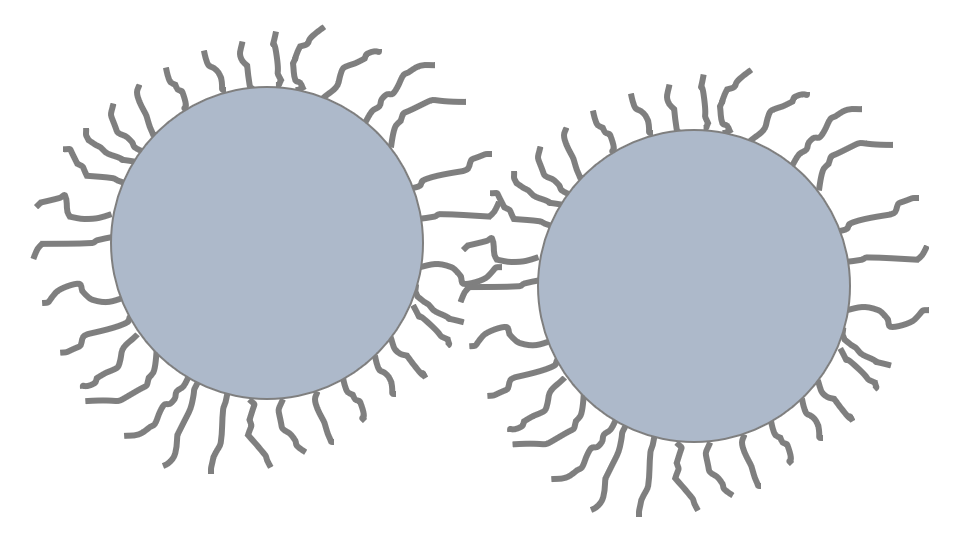
\includegraphics[width=110mm]{chapter1/brushy.PNG}
    \caption{Polymeric brushes on the surface of colloidal particles create steric hindrance, preventing close contact with neighboring particles.}
    \label{fig:brushy}
\end{figure}

These molecular-scale interactions accumulate to define the distance-force relationship between particles in colloidal systems. As the perspective expands from individual particle interactions to larger-scale multi-colloid systems the principles of rheology become increasingly relevant. However, the effects of the microscale lead to the effects seen on the macroscale interactions and as such is critical in understanding the comprehensive behavior of colloidal suspensions. 

\cite{StericForcesReference, PolymerBrushesStudy}


%sedimentation of salt?

\section{Bulk interactions and properties}
%review section

\subsection{Rheology}
Rheology, the study of flow and deformation in materials, is the standard way of examining colloidal systems at the bulk level. In such systems, the clarity of individual particle interactions becomes obscured due to the multitude of forces acting in various directions. These forces, including van der Waals, electrostatic, and steric interactions, govern the dynamics of particles in the colloidal suspension and consequently shape their bulk properties. Rheological techniques, both experimental and through simulations, provide insights into how these individual behaviors accumulate into rheological properties. Oobleck, a well known non-newtonian solution, displays shear thickening properties under shear stress, born from the interplay of forces between the collodial nature of the solution.

\subsection{Non-Newtonian Fluids}
Colloidal particle suspensions often form non-Newtonian fluids. Unlike Newtonian fluids, their behaviors do not conform to Newton's law of viscosity. Instead, their properties arise from the interplay between the particles and the suspending medium. These fluids exhibit intriguing behaviors, such as shear thinning and thickening, which can be attributed to the complex interactions at the particle level.\cite{Rheo2}

Non-Newtonian behavior in colloidal suspensions arises from the complex interplay of these intermolecular forces. For example, in shear thinning, the alignment or structural rearrangement of particles under shear stress reduces internal resistance, a phenomenon deeply rooted in the balance of attractive and repulsive forces at the molecular level.\cite{Rheo2}

\subsection{Shear Thinning and Thickening}
Shear thickening in colloidal suspensions occurs when an increase in shear force leads to an increase in viscosity. Shear thinning consequently is when the same suspension decreases it's viscosity from shear forces. While it may be intuitive to expect that the effects draw from the same mechanical interaction, it has yet to be proven. The current theory is that shear thinning derives from small structural changes in the suspended system. The decrease in viscosity seen in shear thinning emulsions under shear stress can be attributed to the reorientation of particles from reducing the effective area of intermolecular resistance. This reorientation is facilitated by the delicate balance of forces acting at the nanoscale. 

Shear thickening presents a more complex scenario. The addition of salt to a colloidal suspension can suppress electrostatic repulsion between particles, a factor that can significantly influence the transition from shear thinning to thickening. By reducing electrostatic repulsion, salt can promote closer particle interactions, leading to hydroclustering under high shear, resulting in increased viscosity. Where particles form temporary immobilized clusters under compression, and order-to-disorder transitions, where applied forces disrupt the structured flow of particles, increasing viscosity. \cite{hydroshock, ShockCrash}

\subsection{Lubrication Forces}
 This layer is thought to prevent physical contact, and thus frictional forces, between two interacting colloids. From this postulation, the infinite force at R = 0 problem is solved, as the colloids never come into contact, instead separated by thee viscous, lubricating layer between them during floculation. 

Lubrication forces are thought to be the dominant force regarding inter-collodial interactions, causing their observed behaviour and structure (for systems with a high colloidal concentration). These forces arise from thin lubricating layers between particles, preventing direct contact and thus reducing friction. These layers, influenced by van der Waals and electrostatic forces, prevent direct particle contact, facilitating movement and contributing to the unique rheological properties of the suspension. This mechanism potentially resolves the infinite force at $h = 0$ issue in theoretical models, as particles never physically touch but are separated by the lubricating layer. Such forces allow particles to disperse once the applied shear force is removed causing the characteristic shift in viscosity. \cite{LubricationTheoryReference}

This theory assumes spherical particles, which may not always be the case in real systems.\cite{LubricationTheoryReference}

\subsection{Simple Viscous Drag in Colloidal Systems}

Simple viscous drag is a critical aspect of hydrodynamic interactions in colloidal systems. This drag arises from the resistance experienced by colloidal particles as they move through a fluid, heavily influenced by the fluid's viscosity and the particle's velocity. It, along with hydrodynamic forces mentioned before, draws from fluid dynamics, and influences particle movement. With one focusing on individual particle behaviour, and the current focusing on bulk effects. Viscous drag is always in the direction opposite to the motion of the particle, whereas other hydrodynamic forces might have different directions based on flow patterns and particle shape.

This relationship assumes low Reynolds number conditions, where the flow of fluid around the particle is laminar and the effects of inertia are negligible compared to viscous forces.

\subsection{Rheology of suspended collodial particles}

As you scale up the viscosity of a liquid and start applying these forces from the microscale to a collective sum on the macroscale you start to see interesting behaviours arise from the inter-molecular forces.

While Rheology relies on deriving it's understanding of such systems from a macroscopic lense, simulations take the current theory underpinning current scientific understanding to build up a theoretical landscape imitating reality. This in silico landscape often relies on equations use to simulate particle-particle interactions across all of the simulation. Simulations work by drawing a defined box with either periodic or constrained boundary conditions, in two or three dimensions, where each particle's sum force is calculated based upon the other particles within the box. Then, afterwards, the frame of reference is shifted forwards a certain amount of time, with the particle's positions moved based upon the last frame's force. This tick happens over and over, with the total time and accuracy dependant on the delta timestep.\cite{foss_brady_2000}
 
As a result it is important to experimentally verify the results of simulations as the limits of mathematical models can influence the results. As such it is a powerful visualising tool to express how a system is functioning, however, as such it is imperative that the equations used to power this simulation are accurate. 

Experimental verification of these simulations is important, as current models have discussed limitations. Therefore, an experimentalists can contribute to simulations indirectly by verifying and probing the interface of colloids, both in terms of physicality, by directly probing with a cantilever, and probing the interface of theory, by exploring the unknowns of said system.

\cite{SmartMats, Rheo2}


\section{Considering reality}

Whenever considering a mathematical model of reality it is always worth testing it against an assumed case to see whether or not it would hold up. One such case would be to calculate the maximum size of a spherical particle that would retain contact to the roof under its own attractive force, governed by van der Waals interactions.

\subsection{Attaching a marble to the ceiling}

In this instance, lets consider a marble held up to the surface of the ceiling and calculate the maximum size that it would stay there under it own attractive van der Waals forces. Starting from the simple equation of $F = ma$ we simplify our equation down to a rough order of magnitude calculation.


\begin{equation*}
\begin{split}
mg &= F_{\text{vdW}} \\
\rho \frac{4}{3} \pi a^3 g &= \frac{A_H a}{6 h_{m}^2} \\
\rightarrow a &\simeq \sqrt{\frac{3 A_H}{24 \pi \rho g h_{m}^2}} \\
&\simeq \sqrt{\frac{10^{-20} \text{J}}{24 \times 3.14 \times 2500 \text{kg/m}^3 \times 9.81 \text{m/s}^2 \times (10^{-10} \text{m})^2 }} \\
&\simeq 2 \text{mm}
\end{split}
\end{equation*}

In this calculation:

Where $m$ is the mass of the marble, $g$ is the gravitational acceleration, $A_H$ is the Hamaker constant, indicative of the strength of van der Waals forces, $h$ the minimum separation distance between the marble and the ceiling, $p$ is the density of the marble and $a$ is the radius of the marble.

This calculation assumes the marble is a perfect sphere and uses the Hamaker constant to estimate the van der Waals force. The result suggests that a marble of approximately 2 mm radius could adhere to the ceiling under ideal conditions.

%Why did I make this
\begin{figure}[h]     %Insert a figure as soon as possible
        \begin{center}
          \includegraphics[width=110mm]{chapter1/Sphere_on_roof.png}
\end{center}
\caption{A diagram demonstrating a 2mm $radius?? Oh no why is it diameter in the diagram?!$ sphere attached to the ceiling.}
\label{fig:disp}                 % Reference label to the figure.
\end{figure}

Given that the size of the marble is estimated to be approximately 2mm, it seems ludicrous to imagine such a marble staying up against the surface against gravity. However, if you were to imagine 2mm spherical putty, such as Blu tack, against the ceiling, it would be intuitive.

\subsection{Attaching spherical putty to the ceiling}

Contrasting this with the behavior of a sphere of putty, which can adhere to a ceiling, we observe a discrepancy with our thought model. Putty, as a pressure-sensitive adhesive with viscoelastic properties, can conform to surface irregularities, increasing the area of contact and enhancing adhesion. This observation suggests that real-world interactions often involve factors not accounted for in simplified models.

DLVO theory, with its assumption of flat, infinite surfaces and uniformly distributed charges, does not fully encapsulate the complexities of topological variations present in real surfaces. The descent of the DLVO force to infinity at decreasing distances further indicates limitations in its explanatory power. Thus, the deviation from theoretical predictions in practical scenarios like the putty example points to the need for model refinement.

Moreover, as we expand our view from single-particle interactions to systems with multiple interacting entities, the study of rheology becomes pertinent. Rheology, the science of deformation and flow, offers insights into how collective behaviors in multibody systems deviate from simplified theoretical predictions.

This exploration into the practical limitations of theoretical models like DLVO sets the stage for the subsequent investigation using Atomic Force Microscopy (AFM) force curves. AFM provides a nuanced tool to study these interactions at the microscale, offering empirical data to compare against and potentially refine theoretical models.

However, one other consideration can be made about the system described. If a sphere of putty is brought to a ceiling, we know that is capable of adhering to the surface in defiance of gravity. This simple observation lends itself to the consideration that the underlying model is missing a component of reality.

Due to the fact that putty is a pressure-sensitive adhesive, and is viscoelastic, its area of contact is pliable to rough areas. One issue with DLVO theory is that all interacting geometries are assumed to be flat, which is a simplification from reality. As all surfaces in reality are subject to significant topological deviations, DLVO is not always a perfect explanation of the underlying effects. Indeed, all it takes it one look at its descent to infinite force at decreasing distances to see an issue. That being said the question then remains, where does the deviation from reality arise from, and can we incorporate it into the model?

Additionally from these single particle interactions comes a wider array of interactions when the scale of the system expands to accommodate multiple spheres interacting with one another. It is from this simple thought experiment that provides the motivation of this thesis, the pursuit of truth, and the satiation of a simple curiosity. This exploration into the practical limitations of theoretical models like DLVO sets the stage for the subsequent investigation using Atomic Force Microscopy (AFM) force curves. AFM provides a nuanced tool to study these interactions at the microscale, offering empirical data to compare against and potentially refine theoretical models.


\newpage



